 % Chapter Template

\chapter{Results and Discussion}
\label{Chapter5}

We published a web site showing videos and interactive examples to complement this report. It is available at \href{https://distortion.sbovet.ch/}{\textit{distortion.sbovet.ch}}.

As briefly mentioned towards the end of Section \ref{sec:reachableSphere}, the code base used in this project, and particularly the retargeting part implementing the whole Egocentric Coordinate formalism, is problematic. Although well formated and making use of carefully chosen variable names, the code is intrinsically complex and has sadly not been well documented nor commented.

This unfortunately forced us to reconsider the schedule for this project due to issues exposed in a video available on the aforementioned web page. This rescheduling prevented us from performing the experiment described in Chapter \ref{Chapter4} at the time of writing this report. Luckily, we will be able to continue this project in the next six months thanks to a project grant by the Hassler Foundation, hence making it possible to run the experiment and publish its results in a subsequent report.

The remainder of this chapter therefore does not describe the results of the experiment itself, but what we have been able to achieve software-wise in terms of distortion and experiment implementation.

\section{Distortion}

A few examples of distortion and the resulting poses have already been shown on Figures \ref{fig:armExamples} and \ref{fig:divergence}. We propose here a more detailed summary of our results and a discussion of them.


\begin{figure}[h]
    \centering
    \begin{subfigure}[b]{.3\textwidth}
        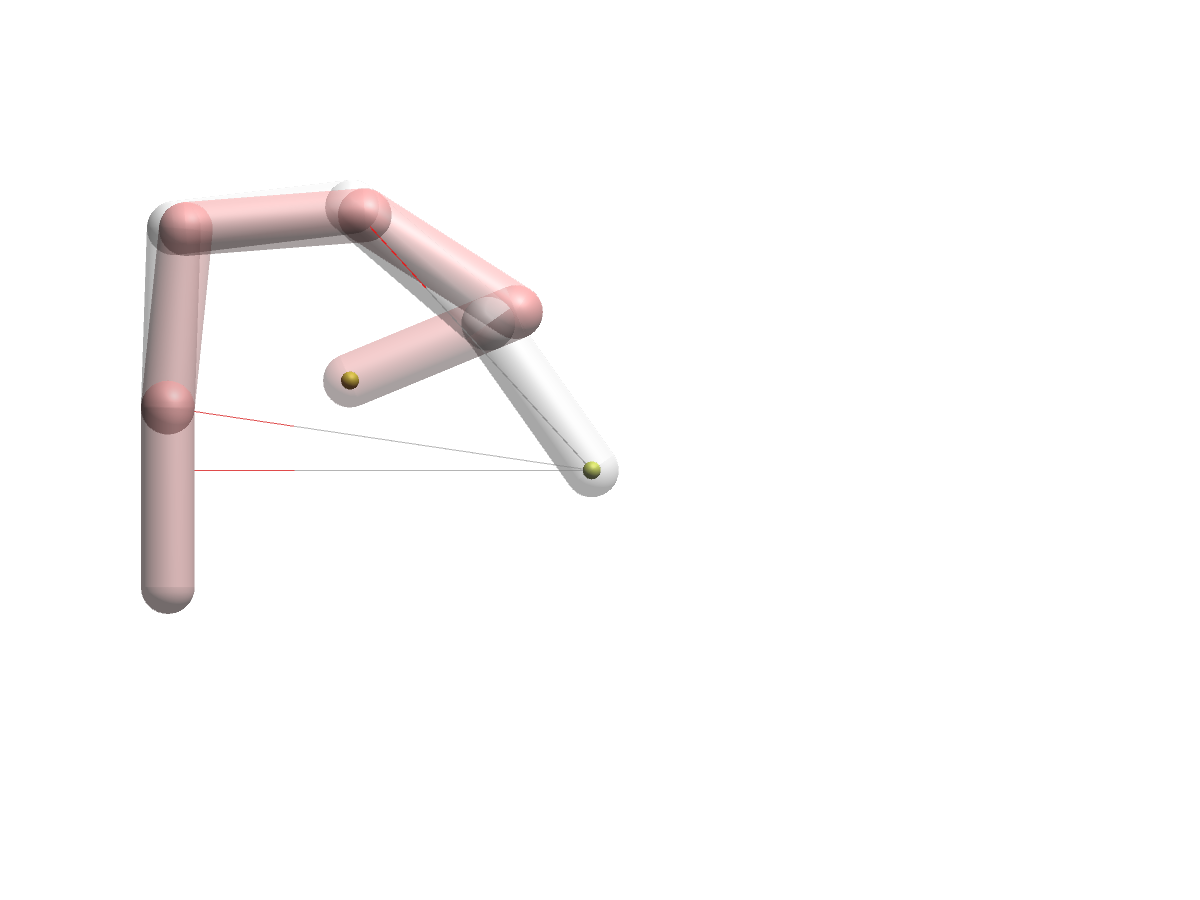
\includegraphics[width=\textwidth]{Figures/distortions/distortions-6.png}
        \caption{$\gamma = -6$}
    \end{subfigure}
    ~
    \begin{subfigure}[b]{.3\textwidth}
        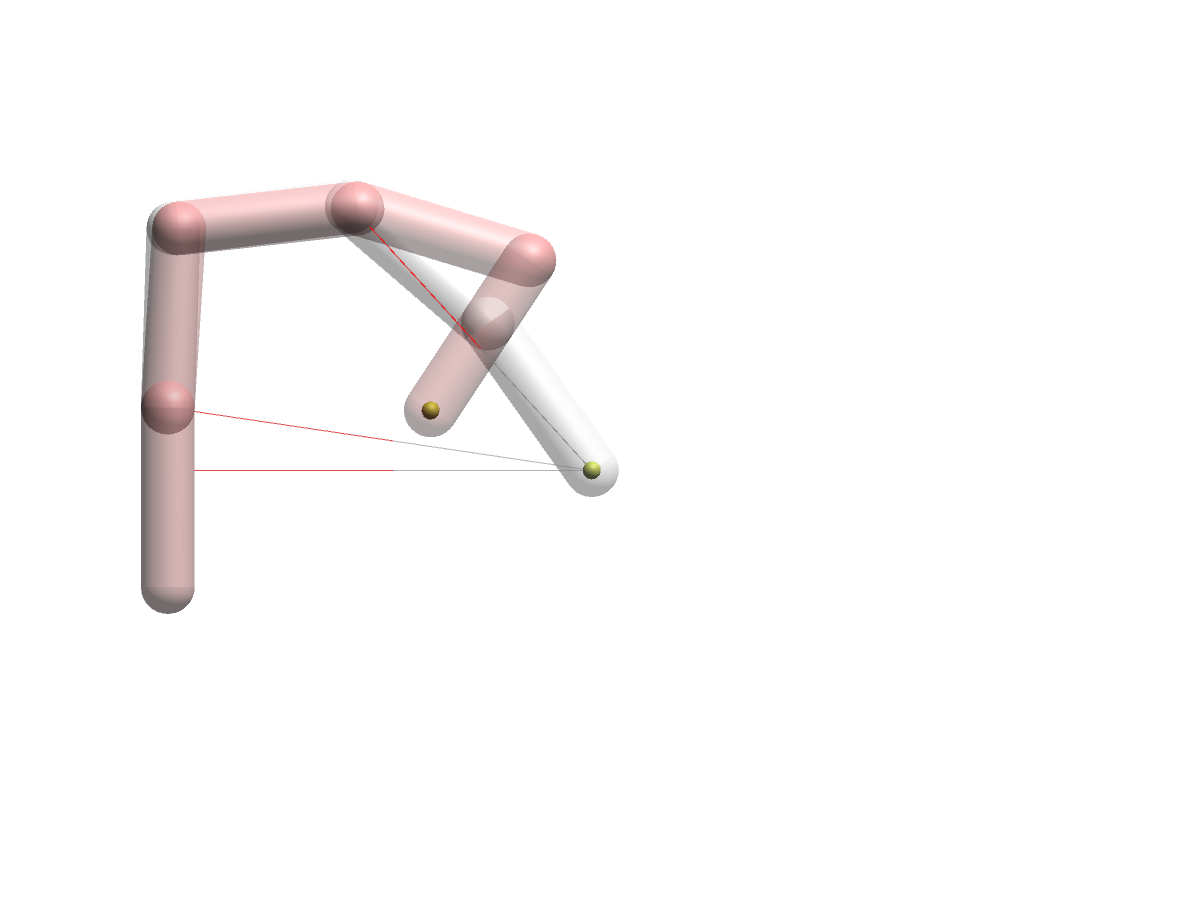
\includegraphics[width=\textwidth]{Figures/distortions/distortions-3.png}
        \caption{$\gamma = -3$}
    \end{subfigure}
    ~
    \begin{subfigure}[b]{.3\textwidth}
        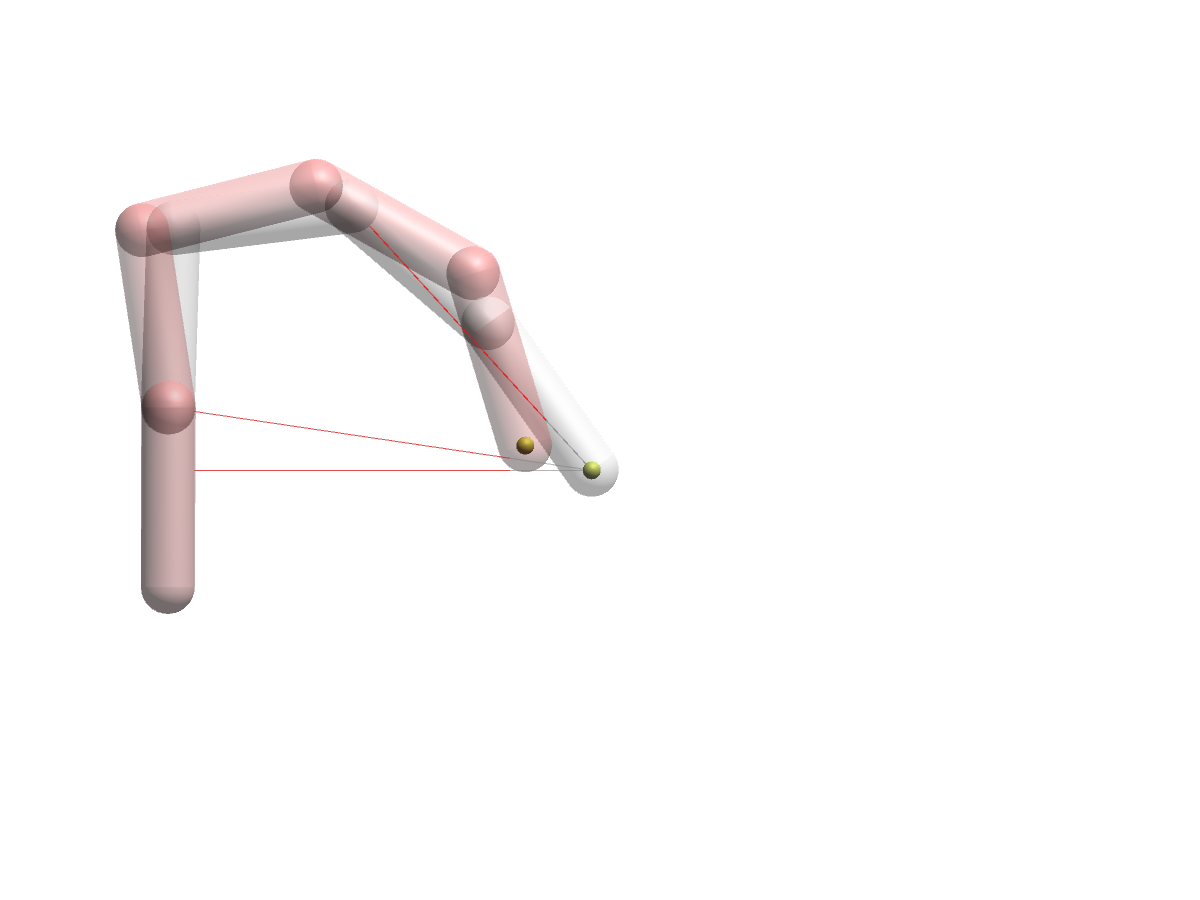
\includegraphics[width=\textwidth]{Figures/distortions/distortions-1.png}
        \caption{$\gamma = -1$}
    \end{subfigure}


    \begin{subfigure}[b]{.3\textwidth}
        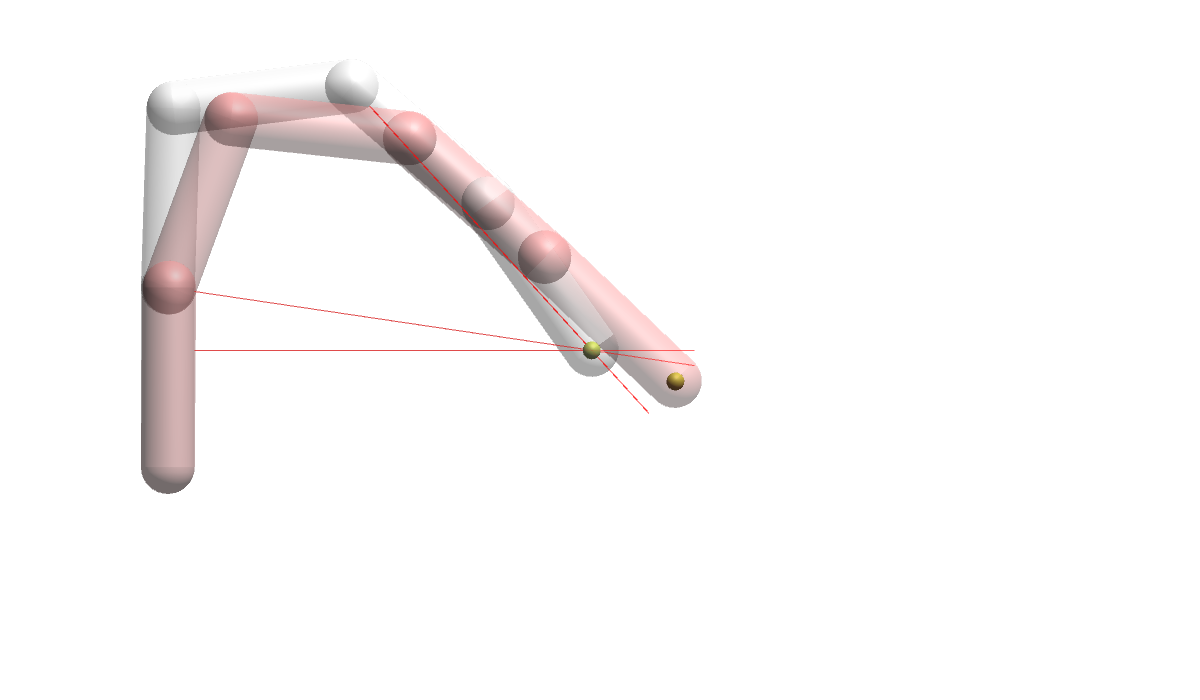
\includegraphics[width=\textwidth]{Figures/distortions/distortions1.png}
        \caption{$\gamma = 1$}
    \end{subfigure}
    ~
    \begin{subfigure}[b]{.3\textwidth}
        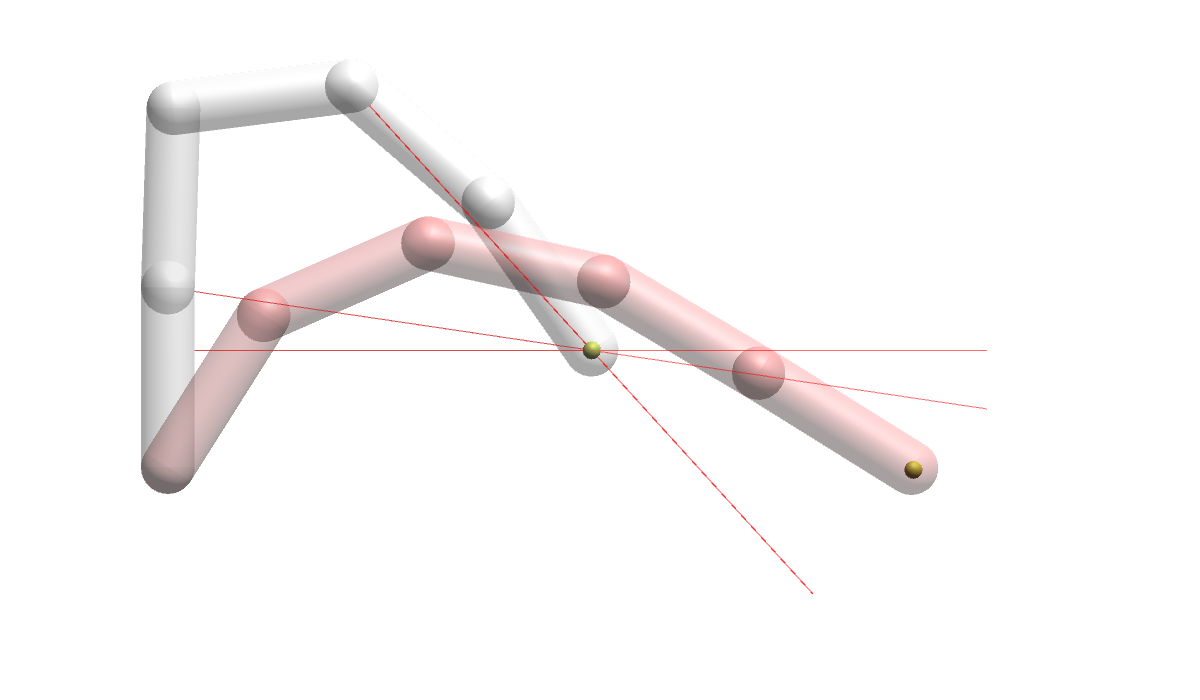
\includegraphics[width=\textwidth]{Figures/distortions/distortions3.png}
        \caption{$\gamma = 3$}
    \end{subfigure}
    ~
    \begin{subfigure}[b]{.3\textwidth}
        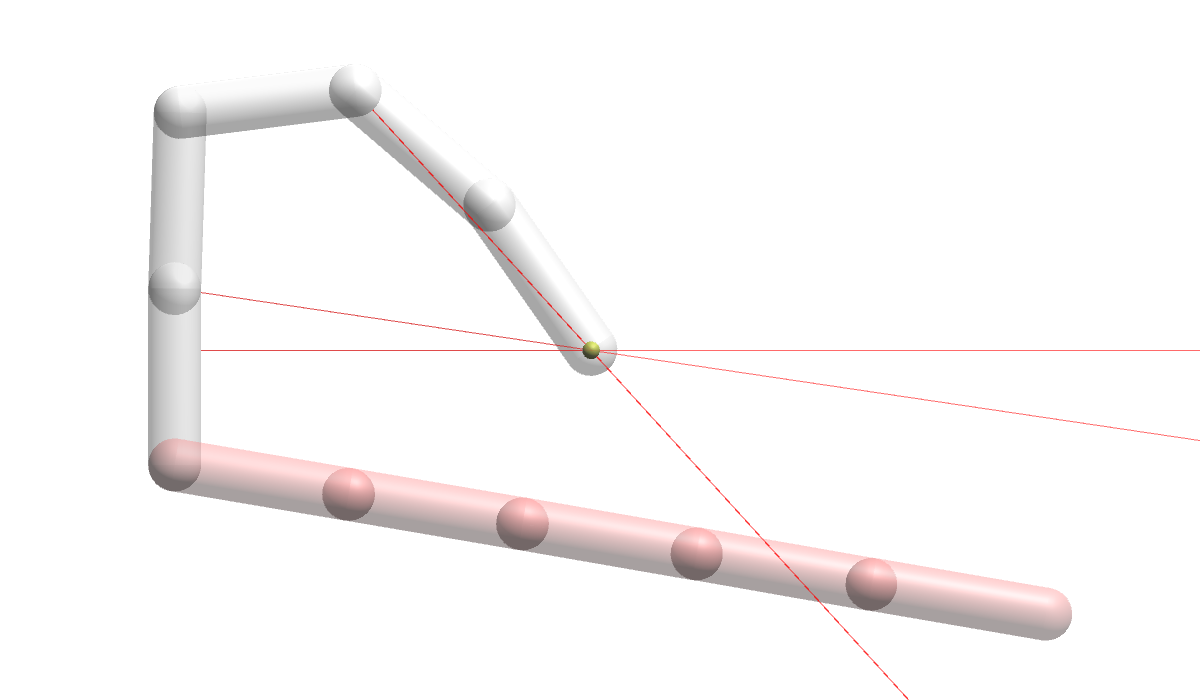
\includegraphics[width=\textwidth]{Figures/distortions/distortions6.png}
        \caption{$\gamma = 6$}
    \end{subfigure}

    \caption{An example of distorted poses. As always, the captured arms are in gray, the distorted ones in red, and the red and gray lines respectively represent the distorted and original Egocentric coordinates.}
    \label{fig:distortionExamples}
\end{figure}

As one can observe on Figure \ref{fig:distortionExamples}, the distortion works the way it is expected to. As a reminder, a gain of $\pm\SI{6}{\decibel}$ corresponds to a movement whose amplitude is respectively multiplied by $3.981$ and $0.251$, which means it is changed almost fourfold in each direction with respect to a non distorted one. A value of $\gamma = \pm\SI{1}{\decibel}$ similarly modifies a movement by $1.259$ or $0.794$.

The behavior of the bottom right arm in Figure \ref{fig:distortionExamples} is precisely the one we proposed to avoid using the reachable sphere described in Section \ref{sec:reachableSphere} but we do not report on it here because, as previously justified, we did not implement it in our experiment.

An interactive web application is available on the web site mentioned above. One may play there with both the real arm position and the gain of the distortion, as well as toggling the presence or not of the reachable sphere. The reader is encouraged to play with the IK chain in order to get a better feeling for how the distortion works, especially how it behaves near the skin.

In order to better understand how such a distortion applies to a captured motion, Figure \ref{fig:realMocapDistortion} shows a subject performing a reaching motion towards the air target. The virtual hand is at the same position on both pictures, but as one may observe, the subject has his hand at different positions. This is due to the fact that in one case (higher hand position) no distortion was applied, while the other (lower hand position) sees a distortion of \SI{3}{\decibel}.

\begin{figure}[h]
    \centering
    \begin{subfigure}[b]{.4\textwidth}
        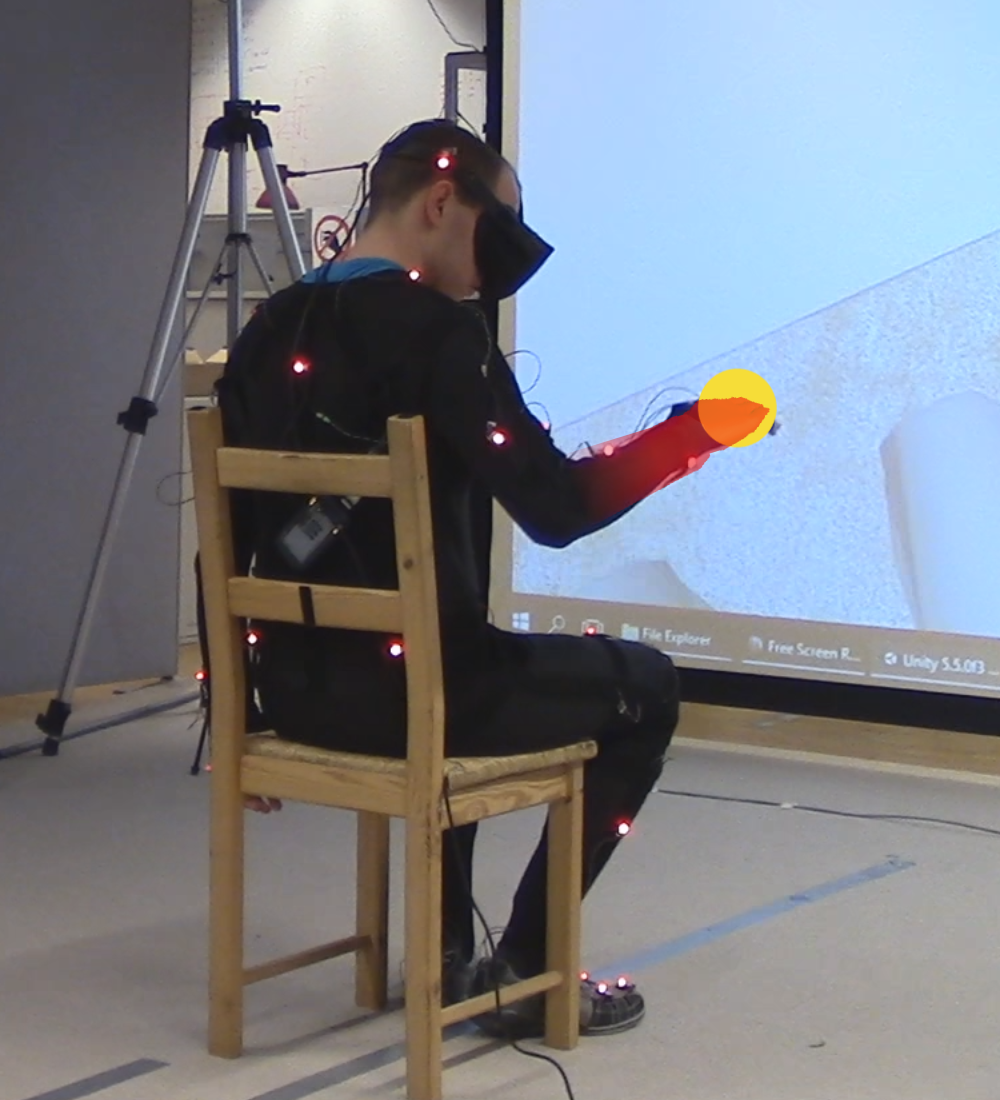
\includegraphics[width=\textwidth]{Figures/handPositionTargetNoDist.png}
    \end{subfigure}
    ~
    \begin{subfigure}[b]{.4\textwidth}
        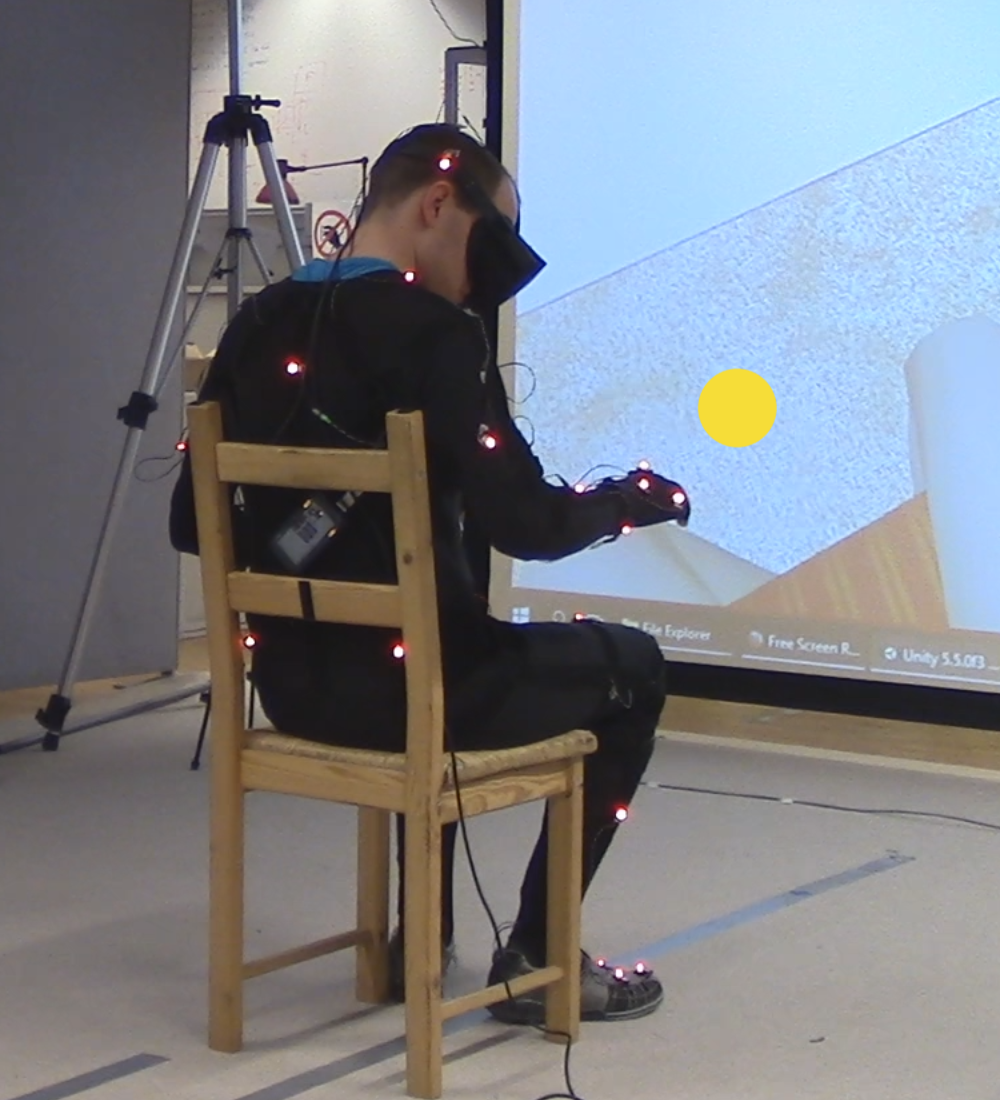
\includegraphics[width=\textwidth]{Figures/handPositionTarget.png}
    \end{subfigure}

    \caption{Pictures of a subject, taken from the same point of view, reaching for the same target but with two different distortions of \SI{0}{\decibel} and \SI{3}{\decibel}, with a visual representation of where the target and virtual hand are (yellow dot and red arm). The left image had no distortion and the right one a distortion of \SI{3}{\decibel}.}
    \label{fig:realMocapDistortion}
\end{figure}

This means that in order to perform the same perceived movement, the subject once had to cover the whole distance between his leg and the target, and could in a second time roughly travel two times less in order to reach the same target.

\section{Experiment}

The aforementioned web site also displays two videos, the first of which is summarizing the experiment process. As stated above, a second video shows some of the issues we encountered towards the end of the project, the resolution of which we will prioritize since these are the only reason we could not perform the experiment at the time of writing this report.

\section{Software Issues}
\label{sec:issues}
As stated at the beginning of this chapter, we encountered some issues during the end of this project. A video entitled `Motion Capture Issues' is available on the website and summarizes said problems.

The first one is a strange torso movement that seem dependent on the angle of both elbows. The camera position is tracked through a different pipeline than the one causing the issue, which has two implications: it avoids any vestibular sensory discrepancy, which is known to cause cybersickness \cite{laviola2000discussion}, but it also causes the torso to have an inconsistent position with respect to the subject's point of view.

A second issue is that of calibration imprecision. Although much a much better calibration process than any previous method we used in the past, it still suffers some imprecisions. The radii of the capsules on each limb segment are for instance computed as the mean of the distance between the previously fitted bone of that limb and the two markers on that limb. For parts such as the thigh, which may sometimes have more of a conic shape, this means that there is slight interpenetrations near the knee and similarly tenuous hovering of the hand towards the hips. While not an issue at all in a typical use case, it becomes problematic when applying a positive distortion to the movements: such small imprecision becomes amplified and one sees much more clearly the error.

Additionally, we currently have an issue with the limbs performing a big jump at a few locations locations near the skin when a positive distortion is applied. For instance when moving outwards from the thigh with constant speed, the virtual hand first jumps a few centimeters before showing a constant speed as well. This issue will most likely cause the subjects to identify a distorted movement much earlier and thus biasing our experiment. We believe it is related to the overlapping of certain body parts, hence the narrow localization of the problem, and will need some further investigation in order to be solved.
